\chapter{Trabalhos Relacionados}

\section{Introdução}

Este capítulo apresenta os trabalhos relacionados à utilização de RNC para treinamento de imagens, com e sem variação de parâmetros; a trabalhos que aplicam especificamente a versão 8 do YOLO; aqueles que utilizaram VANT e os que criaram automação para sistemas de Realidade Virtual. O objetivo é encontrar o estado da arte de cada trabalho, destacando as principais contribuições.

No final do capítulo, os estudos são comparados para justificar o sistema abordado neste trabalho.

\section{Alteração de Parâmetros da RNC}
\subsection{Identificação e Medição de Defeitos em Produtos Automotivos Usando Visão Computacional}

A dissertação apresentada por \cite{gonzaga2023identificaccao} investigou a aplicabilidade e eficiência de um sistema de visão computacional para identificar defeitos visuais no controle de qualidade de peças automotivas reposição. O intuito do trabalho foi de avaliar a possibilidade de automatizar de modo confiável o processo de inspeção e precificação do reparo destas peças.

Para este trabalho, foi utilizado um dataset composto por imagens de vidros automotivos, fornecidos por uma empresa do ramo. Os defeitos analisados incluíram bolhas, delaminação, irisação, ostra e grau em vidros, além de manchas em peças como faróis, lanternas e retrovisores. Todos esses defeitos foram identificados nas fotos fornecidas. Assim como na presente dissertação, foi utilizado o software LabelImg para realizar a marcação da ocorrência de cada uma dessas anomalias no conjunto de fotos, como se vê na Figura \ref{fig:mancha}.

\begin{figure}[!h]
    \center
    \begin{minipage}{0.9\linewidth}
        \center
        \captionsetup{justification=centering,margin=0.5cm,font=small}
        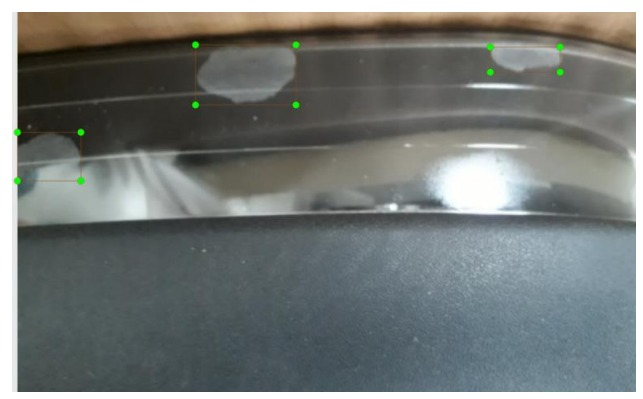
\includegraphics[width=0.7\linewidth]{img/cap3/mancha-marcacao.jpeg}
        \caption{Exemplo de marcação de foto utilizando labelImg, de um defeito em um vidro \cite{gonzaga2023identificaccao}}
        \label{fig:mancha}
    \end{minipage}
\end{figure}

Em sua fundamentação, foram entendidas as RNC como ferramentas eficazes para o processamento de imagens. Avaliou-se a rede ResNet \cite{he2016deep}, como uma possibilidade de arquitetura para processar as imagens, justamente por se mostrar uma ferramenta poderosa para a identificação de padrões. Para tanto, ela se vale de uma série de camadas residuais com conexões de salto, permitindo que os gradientes fluam mais facilmente através da rede durante o treinamento, mitigando o problema do desaparecimento do gradiente. Esse problema ocorre quando, em redes profundas, os gradientes se tornam extremamente pequenos ao retropropagar através das camadas, dificultando a atualização dos pesos nas camadas iniciais e, consequentemente, a aprendizagem adequada da rede. A ResNet supera essa dificuldade utilizando conexões que pulam uma ou mais camadas, somando a entrada diretamente à saída dessas camadas puladas, permitindo a construção de redes muito mais profundas sem a degradação do desempenho (Figura \ref{fig:salto}). Com isso, a ResNet consegue capturar e aprender padrões complexos presentes nas imagens, resultando em uma melhoria significativa na precisão das tarefas de classificação e reconhecimento de imagens.
	
\begin{figure}[!h]
    \center
    \begin{minipage}{0.9\linewidth}
        \center
        \captionsetup{justification=centering,margin=0.5cm,font=small}
        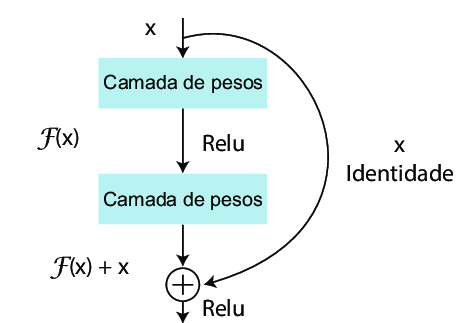
\includegraphics[width=0.7\linewidth]{img/cap3/salto.png}
        \caption{Bloco de aprendizado da ResNet \cite{he2016deep}}
        \label{fig:salto}
    \end{minipage}
\end{figure}

Contudo, a ResNet, devido à sua grande quantidade de camadas e processamento, acaba por ser morosa durante o treinamento. Além disso, sua utilização não é trivial e exige configurações específicas. Deste modo, o trabalho explora as vantagens da YOLO como alternativa. A YOLO é extremamente rápida, treinando em imagens completas com uma única passagem pelas imagens, o que reduz significativamente o tempo de processamento. Sua arquitetura simples e eficiente permite a detecção de múltiplos objetos em uma única passagem pela rede, tornando o treinamento mais direto e eficaz em termos de recursos computacionais. Além disso, a YOLO é altamente generalizável e menos propensa a erros de background, sendo uma solução mais prática e veloz para detecção de objetos.	

Para o treinamento, foram analisadas 3.397 imagens com defeitos específicos da rotina da empresa. Destas, 70\% foram utilizadas para treinamento e 30\% para validação. Todas as imagens foram anotadas manualmente. Em cada uma delas, pelo menos um dos defeitos estudados deveria constar nela para que a imagem fosse colocada para treinamento. Essa parte do processo garantiu que o modelo gerado fosse significativo.

Além disso, foram variados os tamanhos do valor do batch size (entre 2 e 32) e testados três otimizadores diferentes: SGD, Adam e AdamW. A YOLOv5 oferece variações da arquitetura para diferentes propósitos. Neste trabalho, foram testadas 10 variações da arquitetura, juntamente com a alteração de parâmetros. Todos os outros hiperparâmetros foram mantidos na configuração padrão. Cada treinamento foi realizado em 300 épocas.

O otimizador SGD, na variação YOLOv5x, com batch size de 8, alcançou a melhor precisão média, com mAP de 0,72921. Com essa automatização, os testes de aplicação da detecção resultaram em 83,33\% de precisão na precificação correta dos produtos defeituosos (Figura \ref{fig:tabela-macha}).

\begin{figure}[!h]
    \center
    \begin{minipage}{0.9\linewidth}
        \center
        \captionsetup{justification=centering,margin=0.5cm,font=small}
        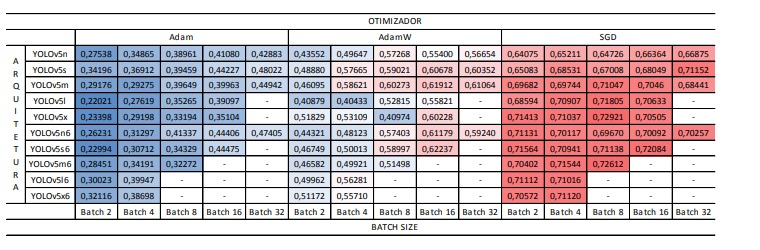
\includegraphics[width=0.7\linewidth]{img/cap3/tabela-mancha.jpeg}
        \caption{Resultado do treinamento variando parâmetros}
        \label{fig:tabela-macha}
    \end{minipage}
\end{figure}


\subsection{Um sistema de prevenção de vazamento de dados de imagens baseado em aprendizado de máquina}

\section{Aplicação YOLOv8}
\subsection{Comparação de Modelos YOLOv5 e YOLOv8 para Detecção de Objetos em Áreas Rurais Usando Transferência de Aprendizado}

No trabalho desenvolvido por \cite{diascomparaccao}, foi realizado "Comparação de Modelos YOLOv5 e YOLOv8 para Detecção de Objetos em Áreas Rurais Usando Transferência de Aprendizado" explora a importância da detecção de objetos em imagens de áreas rurais e compara o desempenho dos modelos YOLOv5 e YOLOv8 neste contexto. A detecção precisa de objetos é crucial para várias aplicações agrícolas, de monitoramento e de preservação ambiental, contribuindo para a eficiência, produtividade e sustentabilidade nas áreas rurais.

Os modelos YOLOv5 e YOLOv8 são abordagens de vanguarda na detecção de objetos em tempo real, cada um com suas próprias características e vantagens. O YOLOv5 demonstrou eficiência no treinamento, enquanto o YOLOv8 se destacou pela precisão na detecção de objetos.

A transferência de aprendizado desempenhou um papel crucial ao adaptar esses modelos pré-treinados para o contexto rural, permitindo que aproveitassem conhecimentos pré-existentes para melhorar o desempenho. Essa abordagem otimiza a eficácia dos modelos, reduzindo significativamente a necessidade de grandes conjuntos de dados e recursos computacionais.

Para trabalhos futuros, sugere-se explorar outras arquiteturas de detecção de objetos, como outras versões da YOLO, Faster R-CNN e Mask R-CNN, para avaliar novas abordagens que possam melhorar ainda mais a precisão e eficiência da detecção de objetos em áreas rurais. Além disso, a incorporação de dados multimodais, como informações de sensores adicionais, imagens de satélite ou dados meteorológicos, pode enriquecer a detecção de objetos em áreas rurais, contribuindo para uma tomada de decisão mais informada e abrangente em setores que dependem dessas informações. A pesquisa contínua nesse campo é essencial para impulsionar a inovação e aprimorar a aplicabilidade da detecção de objetos em áreas rurais.

\subsection{UAV-YOLOv8: A Small-Object-Detection Model Based on Improved YOLOv8 for UAV Aerial Photography Scenarios}

No artigo de \cite{wang2023uav}, é abordada a detecção de objetos pequenos em imagens aéreas capturadas por veículos aéreos não tripulados (VANTs). O problema principal identificado é a baixa precisão dos modelos de detecção de objetos existentes devido à alta proporção de objetos pequenos e aos recursos limitados das plataformas de VANTs.

Para resolver esse problema, os autores propõem o modelo UAV-YOLOv8, uma versão otimizada do YOLOv8. As principais melhorias incluem:

\begin{itemize}
    \item \textbf{Uso do Wise-IoU (WIoU) v3}: Um mecanismo de perda de regressão de caixas delimitadoras que melhora a capacidade de localização do modelo focando em amostras de qualidade comum.
    \item \textbf{Mecanismo de atenção BiFormer}: Otimiza a rede backbone do modelo, aumentando a atenção do modelo para informações críticas.
    \item \textbf{Módulo de processamento de recursos Focal FasterNet Block (FFNB)}: Proporciona uma fusão mais completa de características superficiais e profundas, aumentando o desempenho de detecção e reduzindo a taxa de falhas na detecção de objetos pequenos.
\end{itemize}

Os resultados experimentais mostraram que o UAV-YOLOv8 possui menos parâmetros em comparação com o modelo base, e a precisão média de detecção é 7,7\% maior. Comparado com outros modelos mainstream, o UAV-YOLOv8 demonstrou desempenho superior geral. O estudo utilizou o dataset VisDrone2019, um dos principais conjuntos de dados para fotografia aérea de VANTs, e empregou estratégias de treinamento e métricas de avaliação para validar a eficácia das melhorias propostas.

\section{Inserção automática em Ambientes de Realidade Virtual}
\subsection{Artigo sobre inserção automática...}

\subsection{Subseção 4}

\section{Considerações Finais}

Inserir considerações finais.

\begin{table}[!hbt]
    \centering
    \caption{Resumo comparativo dos trabalhos relacionados}
    \begin{tabular}{ >{\centering\arraybackslash}m{5cm} | >{\centering\arraybackslash}m{2cm} | >{\centering\arraybackslash}m{2cm} | >{\centering\arraybackslash}m{2cm} | >{\centering\arraybackslash}m{2cm} | >{\centering\arraybackslash}m{2cm} }
    \hline
    \cellcolor[gray]{0.9} \textbf{Trabalhos Relacionados} & 
    \cellcolor[gray]{0.9} \begin{sideways} \textbf{Treinamento utilizando YOLOv8} \end{sideways} & 
    \cellcolor[gray]{0.9} \begin{sideways} \textbf{Alteração de Parâmetros da RNC} \end{sideways} & 
    \cellcolor[gray]{0.9} \begin{sideways} \textbf{Utilização de VANT} \end{sideways} & 
    \cellcolor[gray]{0.9} \begin{sideways} \textbf{Subestações de Energia} \end{sideways} &
    \cellcolor[gray]{0.9} \begin{sideways} \textbf{Automação de Inserção de RV} \end{sideways} \\
    \hline 
    \cite{gonzaga2023identificaccao} & \textcolor{green}{\(\checkmark\)} & \textcolor{green}{\(\checkmark\)} & \textcolor{red}{\(\times\)} & \textcolor{red}{\(\times\)} & \textcolor{red}{\(\times\)} \\
    \hline
    \cite{wang2023uav} & \textcolor{green}{\(\checkmark\)} & \textcolor{green}{\(\checkmark\)} & \textcolor{red}{\(\times\)} & \textcolor{red}{\(\times\)} & \textcolor{red}{\(\times\)} \\
    \hline
    \cite{bazame2022detection} & \textcolor{green}{\(\checkmark\)} & \textcolor{green}{\(\checkmark\)} & \textcolor{red}{\(\times\)} & \textcolor{red}{\(\times\)} & \textcolor{red}{\(\times\)} \\
    \end{tabular}
    \label{tab:relacionado1}
\end{table}

A Tabela \ref{tab:relacionado1} apresenta um resumo de todos os trabalhos relacionados descritos neste capítulo, considerando os seguintes temas:

\begin{itemize}
    \item \textit{Treinamento utilizando YOLOv8}: Utilização de RNC para realizar treinamento em conjuntos de imagens;
    \item \textit{Alteração de Parâmetros da RNC para treinamento}: Variação de parâmetros como batch size e otimizadores para treinamento;
    \item \textit{Utilização de VANT}: Coleta de fotos utilizando VANTs;
    \item \textit{Subestações de Energia}: Coleta, treinamento e inserção voltada para subestações de energia;
    \item \textit{Automação de Inserção de RV}: Construção de sistema de inserção automática de objetos em um sistema de RV.
\end{itemize}

Pela análise da Tabela \ref{tab:relacionado1}, é possível notar que, até o presente momento, um sistema que integre todas essas funcionalidades não foi encontrado na literatura. Acredita-se que, através dessas características, o usuário e o terapeuta estarão conectados a um ambiente de treinamento, interagindo de maneira mais natural, segura e eficiente. A ideia é permitir que um usuário, a partir de qualquer lugar com acesso à Internet e a um computador, emita os comandos necessários para controlar um PW, recebendo, ao mesmo tempo, feedback visual aumentado em um dispositivo monitor tradicional. Cada usuário possui diferentes necessidades, e o terapeuta pode configurar um conjunto específico de tarefas que comporão o protocolo de treinamento. Portanto, esta pesquisa propõe a investigação de técnicas computacionais que suportem a integração de todas essas funcionalidades.

No próximo capítulo, serão detalhados os materiais e métodos utilizados para a solução proposta.




